\begin{frame}{On the Agenda}

\begin{itemize}
\tightlist
\item
  Functions

  \begin{itemize}
  \tightlist
  \item
    How to write a function
  \item
    When should we write them?
  \end{itemize}
\item
  Recursion

  \begin{itemize}
  \tightlist
  \item
    Defining something in terms of itself
  \item
    Factorial Calculation (\(n!\))
  \end{itemize}
\item
  Benchmarking

  \begin{itemize}
  \tightlist
  \item
    How fast are you going?
  \end{itemize}
\item
  Memoization

  \begin{itemize}
  \tightlist
  \item
    Caching function calls
  \end{itemize}
\end{itemize}

\end{frame}

\begin{frame}[fragile]{Talking about a Function}

Previously, we just wrote statements like:

\begin{Shaded}
\begin{Highlighting}[]
\KeywordTok{cat}\NormalTok{(}\StringTok{"Hello World!"}\NormalTok{)}
\end{Highlighting}
\end{Shaded}

within a main document.

If we wanted to repeat that phrase elsewhere in the program, we would
have to either:

\begin{enumerate}
\def\labelenumi{\arabic{enumi}.}
\tightlist
\item
  Retype
\item
  Copy and paste
\end{enumerate}

to the new location.

\begin{itemize}
\tightlist
\item
  This is \textbf{not} an ideal situation.
\end{itemize}

\end{frame}

\begin{frame}{What is a Function?}

\textbf{Definition:} A piece of code that performs a specified task that
may or may not depend on parameters and it may or may not return one or
more values.

\begin{center}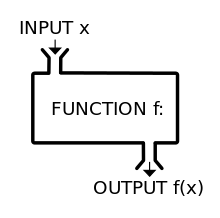
\includegraphics[width=150px]{figures/function_machine} \end{center}

\end{frame}

\begin{frame}{Why use a function?}

Functions are great because:

\begin{enumerate}
\def\labelenumi{\arabic{enumi}.}
\tightlist
\item
  The logic flow is chunked instead of a series of long statements

  \begin{itemize}
  \tightlist
  \item
    Also enables self-documenting depending on the function name.
  \end{itemize}
\item
  Decrease the probability of an error

  \begin{itemize}
  \tightlist
  \item
    Update the code in one central place instead of tracking multiple
    locations

    \begin{itemize}
    \tightlist
    \item
      No need copy code from one section and paste it in another
    \end{itemize}
  \item
    Easily reuse code across multiple analysis
  \item
    No need to understand the internal computation.
  \end{itemize}
\item
  Easier to share code with people that you collaborate.

  \begin{itemize}
  \tightlist
  \item
    Knowledge of what the function \textbf{does}
  \item
    Parameters are established
  \item
    Return information is known
  \end{itemize}
\end{enumerate}

\end{frame}

\begin{frame}{When should I use a function?}

\begin{itemize}
\tightlist
\item
  The moment that you copy and paste more than a line of code within
  your analysis

  \begin{itemize}
  \tightlist
  \item
    This code should be within a function.
  \end{itemize}
\item
  If there is a possibility that you will need to reuse or call the same
  block of code at any point in time, it should be made into a function.
\end{itemize}

\end{frame}

\begin{frame}{Characteristics of a Good Function}

When writing functions, its important not to fall into various traps.
Thus, you should aim for having functions that have:

\begin{enumerate}
\def\labelenumi{\arabic{enumi}.}
\tightlist
\item
  Intuitive Naming Scheme

  \begin{itemize}
  \tightlist
  \item
    Function name and parameters are clear as to their origins.
  \end{itemize}
\item
  Solving a \textbf{single} problem.

  \begin{itemize}
  \tightlist
  \item
    Try to outsource logic so that each step of the problem can be
    analyzed.
  \end{itemize}
\item
  Concise

  \begin{itemize}
  \tightlist
  \item
    Taking many statements and wrapping it into a function should be
    \emph{avoided}.
  \end{itemize}
\end{enumerate}

\end{frame}

\begin{frame}[fragile]{Function Declaration and Calling}

To declare the most simplistic function in R, you must use:

\begin{Shaded}
\begin{Highlighting}[]
\NormalTok{function_name =}\StringTok{ }\NormalTok{function ()  \{}
  \CommentTok{# body}
\NormalTok{\}}
\end{Highlighting}
\end{Shaded}

To call a function, use:

\begin{Shaded}
\begin{Highlighting}[]
\KeywordTok{function_name}\NormalTok{()}
\end{Highlighting}
\end{Shaded}

\end{frame}

\begin{frame}[fragile]{Function Declaration and Call Example}

Here we opt to create a function that will by default say ``Hello
World!''

\begin{Shaded}
\begin{Highlighting}[]
\NormalTok{hello_world =}\StringTok{ }\NormalTok{function() \{ }\CommentTok{# Function Declaration}
  \KeywordTok{cat}\NormalTok{(}\StringTok{"Hello World!}\CharTok{\textbackslash{}n}\StringTok{"}\NormalTok{)    }\CommentTok{# Body Statement}
\NormalTok{\}}

\KeywordTok{hello_world}\NormalTok{()              }\CommentTok{# Call Function}
\end{Highlighting}
\end{Shaded}

\begin{verbatim}
## Hello World!
\end{verbatim}

Notes:

\begin{itemize}
\tightlist
\item
  The function is unable to receive user input.
\item
  Each time the function is called the same result will appear.
\item
  Thus, the function is \textbf{static}.
\end{itemize}

\end{frame}

\begin{frame}[fragile]{Dynamic Function Declaration}

Often times, we will need something more flexible to the ever changing
needs of the world. For a function to be flexible, we must add
\textbf{arguments} to the function.

There are two kinds of arguments:

\begin{itemize}
\tightlist
\item
  \textbf{Positional:} Order matters in the entry
\item
  \textbf{Default Parameter :} Not necessary to specify a value for the
  parameter.
\end{itemize}

\begin{Shaded}
\begin{Highlighting}[]
\NormalTok{func_dynamic =}\StringTok{ }\NormalTok{function (parameter1, }\DataTypeTok{parameter2 =} \OtherTok{NULL}\NormalTok{)  \{}
  \CommentTok{# body}
\NormalTok{\}}
\end{Highlighting}
\end{Shaded}

In this case, \texttt{parameter1} is \emph{positional} and
\texttt{parameter2} is \emph{default parameter}.

\end{frame}

\begin{frame}[fragile]{Dynamic Function Declaration Call}

We can then call the function with either:

\begin{Shaded}
\begin{Highlighting}[]
\CommentTok{# Specify both values}
\KeywordTok{func_dynamic}\NormalTok{(parameter1, paramter2) }

\CommentTok{# Parameter2 will use NULL as the value}
\KeywordTok{func_dynamic}\NormalTok{(parameter1)  }
\end{Highlighting}
\end{Shaded}

\end{frame}

\begin{frame}[fragile]{Dynamic Function Declaration and Call -
Formatting Output}

\textbf{Case Example:} Results need to look presentable and consistent
throughout a document.

\begin{Shaded}
\begin{Highlighting}[]
\CommentTok{# Function Declaration}
\NormalTok{format_percent =}\StringTok{ }\NormalTok{function(x, }\DataTypeTok{digits =} \DecValTok{3}\NormalTok{)\{   }\CommentTok{# Define Func}
  \NormalTok{percent =}\StringTok{ }\KeywordTok{round}\NormalTok{(x *}\StringTok{ }\DecValTok{100}\NormalTok{, }\DataTypeTok{digits =} \NormalTok{digits) }\CommentTok{# Round digits}
  \NormalTok{result =}\StringTok{ }\KeywordTok{paste0}\NormalTok{(percent, }\StringTok{"%"}\NormalTok{)             }\CommentTok{# Add % sign}
  
  \KeywordTok{return}\NormalTok{(result)                            }\CommentTok{# Return}
\NormalTok{\}}
\end{Highlighting}
\end{Shaded}

\end{frame}

\begin{frame}[fragile]{Dynamic Function Declaration and Call -
Formatting Output}

To call the function, we can simply do:

\begin{Shaded}
\begin{Highlighting}[]
\NormalTok{x =}\StringTok{ }\KeywordTok{runif}\NormalTok{(}\DecValTok{5}\NormalTok{)}

\KeywordTok{format_percent}\NormalTok{(x)}
\end{Highlighting}
\end{Shaded}

\begin{verbatim}
## [1] "44.596%" "43.618%" "91.896%" "74.335%" "5.625%"
\end{verbatim}

\begin{Shaded}
\begin{Highlighting}[]
\KeywordTok{format_percent}\NormalTok{(x, }\DataTypeTok{digits =} \DecValTok{0}\NormalTok{)}
\end{Highlighting}
\end{Shaded}

\begin{verbatim}
## [1] "45%" "44%" "92%" "74%" "6%"
\end{verbatim}

\end{frame}

\begin{frame}[fragile]{The Mysterious of \texttt{return()}}

One of the nice aspects of \emph{R}, is you can avoid returning an
object via \texttt{return()} and simply just leave the name of the last
variable.

e.g.

\begin{Shaded}
\begin{Highlighting}[]
\NormalTok{format_percent =}\StringTok{ }\NormalTok{function(x, }\DataTypeTok{digits =} \DecValTok{4}\NormalTok{)\{}
 \NormalTok{percent =}\StringTok{ }\KeywordTok{round}\NormalTok{(x *}\StringTok{ }\DecValTok{100}\NormalTok{, }\DataTypeTok{digits =} \NormalTok{digits)}
 \NormalTok{result =}\StringTok{ }\KeywordTok{paste0}\NormalTok{(percent, }\StringTok{"%"}\NormalTok{)            }

 \NormalTok{result  }\CommentTok{# Last Result}
\NormalTok{\}}
\end{Highlighting}
\end{Shaded}

This will save you \emph{micro}seconds but increase your heartache.

\end{frame}

\begin{frame}[fragile]{The Return Statement}

\begin{Shaded}
\begin{Highlighting}[]
\NormalTok{example_return =}\StringTok{ }\NormalTok{function(}\DataTypeTok{value =} \OtherTok{TRUE}\NormalTok{) \{}
 \NormalTok{if(value) \{}
   \KeywordTok{return}\NormalTok{(}\OtherTok{TRUE}\NormalTok{)  }\CommentTok{# Clear}
 \NormalTok{\} else \{}
   \KeywordTok{return}\NormalTok{(}\OtherTok{FALSE}\NormalTok{) }\CommentTok{# Clear}
 \NormalTok{\}}
\NormalTok{\}}
\end{Highlighting}
\end{Shaded}

\begin{Shaded}
\begin{Highlighting}[]
\NormalTok{example_return =}\StringTok{ }\NormalTok{function(}\DataTypeTok{value =} \OtherTok{TRUE}\NormalTok{) \{}
 \NormalTok{output =}\StringTok{ }\OtherTok{NULL}
 \NormalTok{if(value) \{}
   \NormalTok{output =}\StringTok{ }\OtherTok{TRUE}
 \NormalTok{\} else \{}
   \NormalTok{output =}\StringTok{ }\OtherTok{FALSE}
 \NormalTok{\}}
 \NormalTok{output           }\CommentTok{# Not Clear}
\NormalTok{\}}
\end{Highlighting}
\end{Shaded}

\end{frame}

\begin{frame}[fragile]{The Return Statement}

**\url{Notes:**}

\begin{itemize}
\tightlist
\item
  Harder to read without the \texttt{return} statement
\item
  Requires you \textbf{not} to add any statements after \texttt{output}
\item
  Stick to include \texttt{return} even if the function is a one liner.
\end{itemize}

\end{frame}

\begin{frame}[fragile]{Dynamic Function Declaration and Call -
Formatting Output}

Later, you may wish to add additional features to the function.

To do so, it is recommended that:

\begin{enumerate}
\def\labelenumi{\arabic{enumi}.}
\tightlist
\item
  You use \textbf{default parameter} containing the unmodified value.
\item
  Make sure the function returns similar values.
\end{enumerate}

\begin{Shaded}
\begin{Highlighting}[]
\NormalTok{format_percent =}\StringTok{ }\NormalTok{function(x, }\DataTypeTok{digits =} \DecValTok{4}\NormalTok{, }\DataTypeTok{psign =} \OtherTok{TRUE}\NormalTok{)\{  }
  \NormalTok{percent =}\StringTok{ }\KeywordTok{round}\NormalTok{(x *}\StringTok{ }\DecValTok{100}\NormalTok{, }\DataTypeTok{digits =} \NormalTok{digits) }
  
  \NormalTok{if(psign)\{  }\CommentTok{# Check to see if % should be added}
    \NormalTok{result =}\StringTok{ }\KeywordTok{paste0}\NormalTok{(percent, }\StringTok{"%"}\NormalTok{)}
  \NormalTok{\} else \{}
    \CommentTok{# Coerce to character to match % output.}
    \NormalTok{result =}\StringTok{ }\KeywordTok{as.character}\NormalTok{(percent) }
  \NormalTok{\}}
  \NormalTok{result}
\NormalTok{\}}
\end{Highlighting}
\end{Shaded}

\end{frame}

\begin{frame}{Dynamic Function Declaration and Call - Linear Regression}

Often, when working with linear regression, we want to compute three
different summations to compute other useful diagnostic information:

\begin{itemize}
\tightlist
\item
  The Total Sum of Squares (TSS)
  \[TSS = \sum\limits_{i = 1}^n {{{\left( {{y_i} - {{\bar y}_i}} \right)}^2}}\]
\item
  Fitted Sum of Squares (FSS)
  \[FSS = \sum\limits_{i = 1}^n {{{\left( {{{\hat y}_i} - \bar y} \right)}^2}}\]
\item
  Residual Sum of Squares (RSS)
  \[RSS = \sum\limits_{i = 1}^n {{{\left( {{y_i} - \hat y} \right)}^2}}\]
\end{itemize}

\end{frame}

\begin{frame}[fragile]{Dynamic Function Declaration Example}

Converting these statements to a function yields:

\begin{Shaded}
\begin{Highlighting}[]
\NormalTok{compute_tss =}\StringTok{ }\NormalTok{function (y, y_bar)  \{}
  \KeywordTok{return}\NormalTok{(}\KeywordTok{sum}\NormalTok{( (y -}\StringTok{ }\NormalTok{y_bar)^}\DecValTok{2} \NormalTok{))}
\NormalTok{\}}

\NormalTok{compute_fss =}\StringTok{ }\NormalTok{function (y_hat, y_bar)  \{}
  \KeywordTok{return}\NormalTok{(}\KeywordTok{sum}\NormalTok{( (y_hat -}\StringTok{ }\NormalTok{y_bar)^}\DecValTok{2} \NormalTok{))}
\NormalTok{\}}

\NormalTok{compute_rss =}\StringTok{ }\NormalTok{function (y, y_hat)  \{}
  \KeywordTok{return}\NormalTok{(}\KeywordTok{sum}\NormalTok{( (y -}\StringTok{ }\NormalTok{y_hat)^}\DecValTok{2} \NormalTok{))}
\NormalTok{\}}
\end{Highlighting}
\end{Shaded}

\end{frame}

\begin{frame}{Dynamic Function Declaration and Call - Linear Regression}

These summations have the following relationship:

\[\begin{aligned}
  TSS &= RSS + FSS \\
  \sum\limits_{i = 1}^n {{{\left( {{y_i} - {{\hat y}_i}} \right)}^2}}  &= \sum\limits_{i = 1}^n {{{\left( {{y_i} - \bar y} \right)}^2}}  + \sum\limits_{i = 1}^n {{{\left( {{{\hat y}_i} - \bar y} \right)}^2}}  \\ 
\end{aligned}\]

\end{frame}

\begin{frame}[fragile]{Dynamic Function Declaration - Linear Regression}

Exploiting the previously made functions with the aforementioned
relationship, we get:

\begin{Shaded}
\begin{Highlighting}[]
\NormalTok{tss_relationship =}\StringTok{ }\NormalTok{function (y, y_hat, y_bar)  \{}
  \NormalTok{rss =}\StringTok{ }\KeywordTok{compute_rss}\NormalTok{(y, y_hat)}
  \NormalTok{fss =}\StringTok{ }\KeywordTok{compute_fss}\NormalTok{(y_hat, y_bar)}
  \NormalTok{tss =}\StringTok{ }\NormalTok{rss +}\StringTok{ }\NormalTok{fss}
  \KeywordTok{return}\NormalTok{( tss )}
\NormalTok{\}}
\end{Highlighting}
\end{Shaded}

\end{frame}

\begin{frame}[fragile]{Variable Scope in a Function}

Within a function's \texttt{\{\}}, \emph{R} uses the defined variables
within that region.

\begin{Shaded}
\begin{Highlighting}[]
\NormalTok{multiple_constant =}\StringTok{ }\NormalTok{function(x) \{ }
  \KeywordTok{return}\NormalTok{(value *}\StringTok{ }\NormalTok{x) }\CommentTok{# Note `value` has not been defined.}
\NormalTok{\}}

\CommentTok{# Only on call is an error detected.}
\KeywordTok{multiple_constant}\NormalTok{(}\DecValTok{5}\NormalTok{)}
\NormalTok{## Error in multiple_constant(5) :}
\NormalTok{## object 'value' not found}
\end{Highlighting}
\end{Shaded}

\textbf{Note:}

\begin{itemize}
\tightlist
\item
  \emph{R} always gives you the benefit of the doubt and this sometimes
  gives bad results\ldots{}
\end{itemize}

\end{frame}

\begin{frame}[fragile]{Function vs.~Global Variable Scope}

If a variable is not found, it will search the global environment.

\begin{Shaded}
\begin{Highlighting}[]
\CommentTok{# Define value in global environment}
\CommentTok{# (e.g. outside of the function)}
\NormalTok{value =}\StringTok{ }\DecValTok{3}

\NormalTok{multiple_constant =}\StringTok{ }\NormalTok{function(x) \{ }
  \CommentTok{# `value` is not been defined in the function.}
  \KeywordTok{return}\NormalTok{(value *}\StringTok{ }\NormalTok{x) }
\NormalTok{\}}

\KeywordTok{multiple_constant}\NormalTok{(}\DecValTok{5}\NormalTok{)}
\end{Highlighting}
\end{Shaded}

\begin{verbatim}
## [1] 15
\end{verbatim}

\textbf{Note:}

\begin{itemize}
\tightlist
\item
  This behavior can be very problematic. Try to keep your scope limited.
\end{itemize}

\end{frame}

\begin{frame}[fragile]{Summary of Functions}

\begin{itemize}
\tightlist
\item
  Talked about the steps to creating a function
\item
  The importance behind using \texttt{...}
\item
  Scoping principles as to where R looks.
\end{itemize}

\end{frame}

\begin{frame}{What is Recursion?}

\textbf{Definition:} Defining a process that is in terms of itself such
that the problem is able to be \emph{simplified} and \emph{delegated} in
a reduced state.

Loosely, recursion can be considered in the following light: - If a
problem is easy to solve enough, then simply solve it. - Else, reduce
the problem so that there is \emph{one or more simpler versions} of the
\textbf{same problem} and try to solve them.

\end{frame}

\begin{frame}{Example of Recursion}

Consider the objective of going to
\href{https://www.google.com/maps/place/Illini+Hall,+725+S+Wright+St,+Champaign,+IL+61820/@40.1094428,-88.2314462,17z/data=!3m1!4b1!4m5!3m4!1s0x880cd73f088353ff:0x8d73968b31810cf9!8m2!3d40.1094428!4d-88.2292575}{\textbf{Illini
Hall}}.

Let's define a function called ``Travel to Illini Hall'' and implement
it recursively.

\begin{enumerate}
\def\labelenumi{\arabic{enumi}.}
\tightlist
\item
  If you are in Illini Hall, stop.
\item
  Ask a random person where Illini Hall is and move in the direction
  suggested until you are unsure.
\item
  Travel to Illini Hall
\end{enumerate}

\end{frame}

\begin{frame}{Properties of a Recursive Function}

Inorder for a function to be recursive, it must have the following:

\begin{enumerate}
\def\labelenumi{\arabic{enumi}.}
\tightlist
\item
  \textbf{Base Case}

  \begin{itemize}
  \tightlist
  \item
    Condition to stop
  \item
    Also, the \textbf{simpliest} solution to the problem.
  \end{itemize}
\item
  \textbf{Work} toward \textbf{Base Case}

  \begin{itemize}
  \tightlist
  \item
    Make the problem simplier
  \end{itemize}
\item
  \textbf{Recursive Call}

  \begin{itemize}
  \tightlist
  \item
    Call to itself
  \end{itemize}
\end{enumerate}

\end{frame}

\begin{frame}{Power function}

Another example of recursion would be that of the \textbf{power
function} that acts to simplify repetitve multiplication of one object.

\[\begin{aligned}
  {x^k} &= x \cdot {x^{k - 1}} \\
   &= x \cdot x \cdots x \\
   &= \prod\limits_{i = 1}^k x\\ 
\end{aligned} \]

\end{frame}

\begin{frame}[fragile]{Power Function with Loops}

This behavior can easily be modeled using a loop:

\begin{Shaded}
\begin{Highlighting}[]
\NormalTok{pow_loop =}\StringTok{ }\NormalTok{function(x, n)\{ }\CommentTok{# Define function}
  
  \NormalTok{result =}\StringTok{ }\DecValTok{1}               \CommentTok{# Setup output variable}
  
  \NormalTok{for(i in }\KeywordTok{seq_len}\NormalTok{(n))\{    }\CommentTok{# Loop over the power}
    \NormalTok{result =}\StringTok{ }\NormalTok{result*x}
  \NormalTok{\}}
  
  \NormalTok{result                   }\CommentTok{# Return the result}
\NormalTok{\}}
\end{Highlighting}
\end{Shaded}

\textbf{Note:} This implementation does \emph{not} support negative
exponents!

\end{frame}

\begin{frame}[fragile]{Power Function with Recursion}

However, we're more interested in recursively defining the function.

That is, we want to define the power function in terms of \emph{itself}.

\begin{Shaded}
\begin{Highlighting}[]
\NormalTok{pow =}\StringTok{ }\NormalTok{function(x, n)\{ }\CommentTok{# Define function}
  
    \NormalTok{if (n <=}\StringTok{ }\DecValTok{0}\NormalTok{)\{      }\CommentTok{# Set a base case}
      \KeywordTok{return}\NormalTok{(}\DecValTok{1}\NormalTok{)       }\CommentTok{# No recursive call}
    \NormalTok{\} }
    
    \CommentTok{# Solve a small part of the larger problem}
    \KeywordTok{return}\NormalTok{(x *}\StringTok{ }\KeywordTok{pow}\NormalTok{(x, n -}\StringTok{ }\DecValTok{1}\NormalTok{)) }\CommentTok{# Call ourself}
\NormalTok{\}}
\end{Highlighting}
\end{Shaded}

\textbf{Note:} This implementation does \emph{not} support negative
exponents!

\end{frame}

\begin{frame}[fragile]{Behind the Scenes of the Power Function in R}

What we are saying in this particular case is that:

\begin{itemize}
\tightlist
\item
  \texttt{pow(x,\ n)\ =\ x*pow(x,\ n\ -\ 1)}
\end{itemize}

So that, if \texttt{pow(2,5)}, we have:

\begin{itemize}
\tightlist
\item
  \texttt{pow(2,5)} is equal to \texttt{x\ *\ pow(2,4)}
\item
  \texttt{pow(2,4)} is equal to \texttt{x\ *\ pow(2,3)}
\item
  \texttt{pow(2,3)} is equal to \texttt{x\ *\ pow(2,2)}
\item
  \texttt{pow(2,2)} is equal to \texttt{x\ *\ pow(2,1)}
\item
  \texttt{pow(2,1)} is equal to \texttt{x\ *\ pow(2,0)}
\item
  \texttt{pow(2,0)} is equal to \texttt{1}
\end{itemize}

That is, we have broken down each of the components to obtain the power
and have end up with the solution. The key is the last stage of the
problem, where we invoke the base case to stop the recursion.

\end{frame}

\begin{frame}[fragile]{Viewing Recursion from a Functional Perspective}

\begin{Shaded}
\begin{Highlighting}[]
\NormalTok{pow =}\StringTok{ }\NormalTok{function(x, n, d)\{ }\CommentTok{# Define function}
    \CommentTok{# Add a tracer into the function}
    \NormalTok{spacer =}\StringTok{ ""}\NormalTok{; }
    \NormalTok{for (i in }\KeywordTok{seq_len}\NormalTok{(d)) \{}
        \NormalTok{spacer =}\StringTok{ }\KeywordTok{paste0}\NormalTok{(spacer, }\StringTok{" "}\NormalTok{, }\DataTypeTok{collapse =} \StringTok{""}\NormalTok{)}
    \NormalTok{\}}
    \KeywordTok{cat}\NormalTok{(spacer, }\StringTok{"pow("}\NormalTok{,x,}\StringTok{","}\NormalTok{,n,}\StringTok{")}\CharTok{\textbackslash{}n}\StringTok{"}\NormalTok{, }\DataTypeTok{sep=}\StringTok{""}\NormalTok{)}

    \CommentTok{# --------- Same code as before}
    
    \NormalTok{if (n <=}\StringTok{ }\DecValTok{0}\NormalTok{)\{       }\CommentTok{# Set a base case}
      \KeywordTok{return}\NormalTok{(}\DecValTok{1}\NormalTok{)       }\CommentTok{# No recursive call}
    \NormalTok{\} }
    
    \CommentTok{# Solve a small part of the larger problem}
    \KeywordTok{return}\NormalTok{(x *}\StringTok{ }\KeywordTok{pow}\NormalTok{(x, n -}\StringTok{ }\DecValTok{1}\NormalTok{, d +}\StringTok{ }\DecValTok{4}\NormalTok{)) }\CommentTok{# Call ourself}
\NormalTok{\}}
\end{Highlighting}
\end{Shaded}

\end{frame}

\begin{frame}[fragile]{Viewing recursion from a functional perspective}

\begin{Shaded}
\begin{Highlighting}[]
\KeywordTok{cat}\NormalTok{(}\KeywordTok{pow}\NormalTok{(}\DecValTok{7}\NormalTok{, }\DecValTok{2}\NormalTok{, }\DecValTok{0}\NormalTok{))}
\end{Highlighting}
\end{Shaded}

\begin{verbatim}
## pow(7,2)
##     pow(7,1)
##         pow(7,0)
## 49
\end{verbatim}

\end{frame}

\begin{frame}{Factorials}

A more useful recursive function is that of a \textbf{factorial}.

Factorials are given by:

\[\begin{aligned}
  n! &= n \cdot \left( {n - 1} \right)!  \\
   &= n\left( {n - 1} \right)\left( {n - 2} \right) \cdots 3 \cdot 2 \cdot 1  \\
   &= \prod\limits_{i = 1}^n i   \\ 
\end{aligned}\]

\textbf{Note:} Consider viewing
\href{http://thecoatlessprofessor.com/statistics/proofs-of-gamma-distribution/}{Proofs
of the Gamma distribution} to understand the recursive nature of the
Gamma function for integers \(n! = \Gamma \left( {n + 1} \right)\)

\end{frame}

\begin{frame}{Use cases}

\textbf{Factorials} are commonly used in Combinatorics for:

\begin{itemize}
\tightlist
\item
  \textbf{Permutations:} Order of selection matters without replication
\end{itemize}

\[P\left( {n,k} \right) = \frac{{n!}}{{\left( {n - k} \right)!}}\]

\begin{itemize}
\tightlist
\item
  \textbf{Combinations:} Order of selection does not matter without
  replication
\end{itemize}

\[\begin{aligned}
C\left( {n,k} \right) &=\left( \begin{gathered}
  n  \\
  k  \\ 
\end{gathered}  \right) \\
&=  \frac{{P\left( {n,k} \right)}}{{P\left( {k,k} \right)}} \\
&= \frac{{n!}}{{k!\left( {n - k} \right)!}}
\end{aligned}\]

\end{frame}

\begin{frame}[fragile]{Factorial}

Here is a custom implementation of the factorial function:

\begin{Shaded}
\begin{Highlighting}[]
\NormalTok{factorial_r <-}\StringTok{ }\NormalTok{function(x)\{    }\CommentTok{# Function Definition}
  \NormalTok{if(x <=}\StringTok{ }\DecValTok{1}\NormalTok{)\{}
    \KeywordTok{return}\NormalTok{(}\DecValTok{1}\NormalTok{)}
  \NormalTok{\} else \{}
    \KeywordTok{return}\NormalTok{(x*}\KeywordTok{factorial_r}\NormalTok{(x}\DecValTok{-1}\NormalTok{))}
  \NormalTok{\}}
\NormalTok{\}}
\end{Highlighting}
\end{Shaded}

\begin{itemize}
\tightlist
\item
  Identify the 3 parts of the recursive algorithm
\end{itemize}

\textbf{Note:} Factorials in \emph{R} are given by the
\texttt{factorial(x)} function and not \texttt{!x} (Why?)

\end{frame}

\begin{frame}{Misc note on Recursion}

\begin{itemize}
\tightlist
\item
  Examples provided deal with \textbf{tail} recursion.

  \begin{itemize}
  \tightlist
  \item
    That is, the last statement of the function is calling itself.
  \end{itemize}
\item
  Only \textbf{tail} recursion can be converted to using \textbf{loops}.
\item
  \textbf{Avoid}, like the plauge, using \textbf{global variables} with
  recursion.
\end{itemize}

\end{frame}

\begin{frame}{Summary on Recursion}

\begin{itemize}
\tightlist
\item
  Recursive functions call themselves
\item
  Recursion exists in everyday statistics
\end{itemize}

\end{frame}

\begin{frame}{Benchmarking}

Coming up next\ldots{} \textbf{Benchmarking} in R!

\end{frame}

\begin{frame}{Code Implementations}

\begin{itemize}
\tightlist
\item
  There are many ways to implement an idea..

  \begin{itemize}
  \tightlist
  \item
    The question is:
  \item
    What implementation is the best?
  \end{itemize}
\end{itemize}

\end{frame}

\begin{frame}{Benchmark}

To answer what implementation works the best, one needs to employ a
benchmark to obtain \textbf{quantifiable results}.

Benchmarks are an ideal way to quantify how well a method performs
because it has the ability to:

\begin{enumerate}
\def\labelenumi{\arabic{enumi}.}
\tightlist
\item
  Show the amount of time the code has been running
\item
  Bottlenecks
\item
  Sloppy coding
\end{enumerate}

Plus, it appeals to our quest for data driven decisions.

\end{frame}

\begin{frame}{A Note on Benchmarks..}

Benchmarks are like a microscope.

\begin{center}
\includegraphics[width=150px]{figures/microscope} \end{center}

Magnification is able to be adjusted\ldots{} But what are you really
observing?

The truth? Or just a clever lie?

\end{frame}

\begin{frame}{Writing a Benchmark}

Benchmarks can be very tempting to use to solely make decisions.

However, in order for the benchmark to be beneficial, the benchmark must
be done properly.

\end{frame}

\begin{frame}{Properly Writing a Benchmark}

To ensure the code is properly time benchmarked, do the following:

\begin{enumerate}
\def\labelenumi{\arabic{enumi}.}
\tightlist
\item
  Only have R open
\item
  Do not use the computer while the benchmark is active.
\item
  Warm up code prior to benchmarking (code will be ``hot'' during
  benchmark)
\item
  Have enough replications (N = 100)
\item
  Fix the data used per replication (e.g.~same seed)
\item
  Check code provides same output
\end{enumerate}

With this being said, let's create one (or two) to see how it works!

\end{frame}

\begin{frame}[fragile]{The Simpliest Benchmark}

The simpliest benchmark is given with R's built in
\texttt{system.time()} function.

The key time is the ``elapsed'' time as it is the summation of the
others.

\begin{Shaded}
\begin{Highlighting}[]
\NormalTok{out =}\StringTok{ }\KeywordTok{system.time}\NormalTok{(\{}\KeywordTok{Sys.sleep}\NormalTok{(}\DecValTok{1}\NormalTok{)\})}
\NormalTok{out}
\end{Highlighting}
\end{Shaded}

\begin{verbatim}
##    user  system elapsed 
##   0.001   0.000   1.005
\end{verbatim}

\begin{Shaded}
\begin{Highlighting}[]
\NormalTok{out[}\DecValTok{3}\NormalTok{]}
\end{Highlighting}
\end{Shaded}

\begin{verbatim}
## elapsed 
##   1.005
\end{verbatim}

\textbf{Note:} Adding, removing, or modifying a variable will impact the
timing!

\end{frame}

\begin{frame}[fragile]{Setting the Stage}

In this case, we are going to be interested in two ideas:

\begin{enumerate}
\def\labelenumi{\arabic{enumi}.}
\tightlist
\item
  The cost of operating on a \texttt{matrix} vs.~a \texttt{dataframe}.
\item
  The cost of using () vs \{\}. (Credit to
  \href{http://dirk.eddelbuettel.com/blog/2011/04/12/}{Dirk
  Eddelbuettel})
\end{enumerate}

\end{frame}

\begin{frame}[fragile]{Setting the Stage}

For the first benchmark case, we are going to create the following
objects:

\begin{Shaded}
\begin{Highlighting}[]
\CommentTok{# Set seed for reproducibility}
\KeywordTok{set.seed}\NormalTok{(}\DecValTok{1337}\NormalTok{)}

\CommentTok{# Construct large matrix object}
\NormalTok{matrix.op =}\StringTok{ }\KeywordTok{matrix}\NormalTok{(}\KeywordTok{rnorm}\NormalTok{(}\DecValTok{10000}\NormalTok{*}\DecValTok{100}\NormalTok{), }\DecValTok{10000}\NormalTok{, }\DecValTok{100}\NormalTok{)}

\CommentTok{# Convert matrix object to data.frame}
\NormalTok{dataframe.op =}\StringTok{ }\KeywordTok{as.data.frame}\NormalTok{(matrix.op)}
\end{Highlighting}
\end{Shaded}

\end{frame}

\begin{frame}[fragile]{Cost of using Parentheses vs.~Curly Brackets}

\begin{Shaded}
\begin{Highlighting}[]
\CommentTok{# Different R implementations}
\NormalTok{f =}\StringTok{ }\NormalTok{function(n, }\DataTypeTok{x=}\DecValTok{1}\NormalTok{) for (i in }\DecValTok{1}\NormalTok{:n) x=}\DecValTok{1}\NormalTok{/(}\DecValTok{1}\NormalTok{+x)}
\NormalTok{g =}\StringTok{ }\NormalTok{function(n, }\DataTypeTok{x=}\DecValTok{1}\NormalTok{) for (i in }\DecValTok{1}\NormalTok{:n) x=(}\DecValTok{1}\NormalTok{/(}\DecValTok{1}\NormalTok{+x))}
\NormalTok{h =}\StringTok{ }\NormalTok{function(n, }\DataTypeTok{x=}\DecValTok{1}\NormalTok{) for (i in }\DecValTok{1}\NormalTok{:n) x=(}\DecValTok{1}\NormalTok{+x)^(-}\DecValTok{1}\NormalTok{)}
\NormalTok{j =}\StringTok{ }\NormalTok{function(n, }\DataTypeTok{x=}\DecValTok{1}\NormalTok{) for (i in }\DecValTok{1}\NormalTok{:n) x=\{}\DecValTok{1}\NormalTok{/\{}\DecValTok{1}\NormalTok{+x\}\}}
\NormalTok{k =}\StringTok{ }\NormalTok{function(n, }\DataTypeTok{x=}\DecValTok{1}\NormalTok{) for (i in }\DecValTok{1}\NormalTok{:n) x=}\DecValTok{1}\NormalTok{/\{}\DecValTok{1}\NormalTok{+x\}}
\end{Highlighting}
\end{Shaded}

\end{frame}

\begin{frame}[fragile]{Cost of using Parentheses vs.~Curly Brackets}

To illustrate the benefits of compiler vs.~interpreter, we're also going
to call upon C++ using Rcpp.

Do not worry about understanding the code presented next\ldots{}

\begin{Shaded}
\begin{Highlighting}[]
\CommentTok{# Load Rcpp}
\KeywordTok{library}\NormalTok{(Rcpp)}

\CommentTok{# Define a version in C++ called }
\KeywordTok{cppFunction}\NormalTok{(}\DataTypeTok{code=}\StringTok{'int d(int n, double x = 1.0)\{}
\StringTok{                  for (int i=0; i<n; i++) x=1/(1+x);}
\StringTok{                  return x;}
\StringTok{                  \}'}\NormalTok{)}
\end{Highlighting}
\end{Shaded}

\end{frame}

\begin{frame}[fragile]{R Package: rbenchmark}

The \texttt{rbenchmark} R package provides a way to obtain the total
amount of time elapsed for a given piece of code run over \(N\)
replications.

The benchmark is initiated by:

\begin{verbatim}
# Load Library
library('rbenchmark')

# Run benchmark
benchmark(testfun1 = somefun(),
          testfun2 = otherfun())
\end{verbatim}

\end{frame}

\begin{frame}{R Package: rbenchmark}

The results returned are:

\begin{itemize}
\tightlist
\item
  The user, system, and total elapsed times for the active R process
\item
  The cumulative sum of user and system times of any child processes
  spawned by it on which it has waited. (\emph{.child, }.self)
\end{itemize}

\end{frame}

\begin{frame}[fragile]{R Package: \texttt{rbenchmark} - Case 1}

\begin{Shaded}
\begin{Highlighting}[]
\CommentTok{# Load Library}
\KeywordTok{library}\NormalTok{(}\StringTok{'rbenchmark'}\NormalTok{)}

\CommentTok{# Run benchmark}
\NormalTok{out =}\StringTok{ }\KeywordTok{benchmark}\NormalTok{(}\DataTypeTok{mat.op =} \KeywordTok{apply}\NormalTok{(matrix.op, }\DecValTok{2}\NormalTok{, sd), }
                \DataTypeTok{df.op =} \KeywordTok{apply}\NormalTok{(dataframe.op, }\DecValTok{2}\NormalTok{, sd))}

\CommentTok{# Table Object}
\NormalTok{out}
\end{Highlighting}
\end{Shaded}

\begin{verbatim}
##     test replications elapsed relative user.self sys.self user.child
## 2  df.op          100   5.659    2.484     4.747    0.202          0
## 1 mat.op          100   2.278    1.000     2.008    0.114          0
##   sys.child
## 2         0
## 1         0
\end{verbatim}

\begin{Shaded}
\begin{Highlighting}[]
\CommentTok{# Average time spent per iteration}
\NormalTok{out[,}\StringTok{"elapsed"}\NormalTok{]/out[,}\StringTok{"replications"}\NormalTok{]}
\end{Highlighting}
\end{Shaded}

\begin{verbatim}
## [1] 0.05659 0.02278
\end{verbatim}

\end{frame}

\begin{frame}[fragile]{R Package: \texttt{rbenchmark} - Case 2}

\begin{Shaded}
\begin{Highlighting}[]
\NormalTok{N =}\StringTok{ }\FloatTok{1e6} \CommentTok{# Number of Times to Run Loop}
\NormalTok{out =}\StringTok{ }\KeywordTok{benchmark}\NormalTok{(}\KeywordTok{f}\NormalTok{(N, }\DecValTok{1}\NormalTok{), }\KeywordTok{g}\NormalTok{(N, }\DecValTok{1}\NormalTok{), }\KeywordTok{h}\NormalTok{(N, }\DecValTok{1}\NormalTok{), }\KeywordTok{j}\NormalTok{(N, }\DecValTok{1}\NormalTok{), }\KeywordTok{k}\NormalTok{(N, }\DecValTok{1}\NormalTok{), }\KeywordTok{d}\NormalTok{(N, }\DecValTok{1}\NormalTok{), }\CommentTok{# Test Funcs}
          \DataTypeTok{columns =} \KeywordTok{c}\NormalTok{(}\StringTok{"test"}\NormalTok{, }\StringTok{"replications"}\NormalTok{, }\StringTok{"elapsed"}\NormalTok{, }\StringTok{"relative"}\NormalTok{), }
          \DataTypeTok{order=}\StringTok{"relative"}\NormalTok{,  }\CommentTok{# Order the results by speed (lower is better)}
          \DataTypeTok{replications=}\DecValTok{20}\NormalTok{)   }\CommentTok{# Number of runs for each function}
\end{Highlighting}
\end{Shaded}

\begin{longtable}[c]{@{}llrrr@{}}
\toprule
& test & replications & elapsed & relative\tabularnewline
\midrule
\endhead
6 & d(N, 1) & 20 & 0.184 & 1.000\tabularnewline
5 & k(N, 1) & 20 & 5.705 & 31.005\tabularnewline
1 & f(N, 1) & 20 & 5.925 & 32.201\tabularnewline
4 & j(N, 1) & 20 & 6.621 & 35.984\tabularnewline
2 & g(N, 1) & 20 & 7.383 & 40.125\tabularnewline
3 & h(N, 1) & 20 & 9.964 & 54.152\tabularnewline
\bottomrule
\end{longtable}

\end{frame}

\begin{frame}[fragile]{R Package: \texttt{rbenchmark} - Case 2}

The average amount of time a replication takes can be obtained via:

\begin{Shaded}
\begin{Highlighting}[]
\NormalTok{out[,}\StringTok{"elapsed"}\NormalTok{] /}\StringTok{ }\NormalTok{out[,}\StringTok{"replications"}\NormalTok{]}
\end{Highlighting}
\end{Shaded}

\begin{verbatim}
## [1] 0.00920 0.28525 0.29625 0.33105 0.36915 0.49820
\end{verbatim}

\end{frame}

\begin{frame}[fragile]{Drilling down with \texttt{microbenchmark}}

\begin{itemize}
\tightlist
\item
  The \texttt{microbenchmark} R package provides a way to record time
  for each iteration unsummed!

  \begin{itemize}
  \tightlist
  \item
    This provides more magnification on functions than
    \texttt{rbenchmark}.
  \end{itemize}
\item
  To use \texttt{microbenchmark} do the following:
\end{itemize}

\begin{Shaded}
\begin{Highlighting}[]
\CommentTok{# Load Library}
\KeywordTok{library}\NormalTok{(}\StringTok{'microbenchmark'}\NormalTok{)}

\CommentTok{# Run benchmark}
\KeywordTok{microbenchmark}\NormalTok{(}\DataTypeTok{testfun1 =} \KeywordTok{somefun}\NormalTok{(), }\CommentTok{# List Functions}
               \DataTypeTok{testfun2 =} \KeywordTok{otherfun}\NormalTok{(), }
               \DataTypeTok{times =} \DecValTok{100}\NormalTok{) }\CommentTok{# Number of Replications}
\end{Highlighting}
\end{Shaded}

\textbf{Note:} This is not ideal for large functions. This is meant for
pinpoint precision of elements.

\end{frame}

\begin{frame}[fragile]{Drilling down with \texttt{microbenchmark} - Case
1}

\begin{Shaded}
\begin{Highlighting}[]
\CommentTok{# Load Library}
\KeywordTok{library}\NormalTok{(}\StringTok{'microbenchmark'}\NormalTok{)}

\CommentTok{# Run benchmark}
\NormalTok{out =}\StringTok{ }\KeywordTok{microbenchmark}\NormalTok{(}\DataTypeTok{mat.op =} \KeywordTok{apply}\NormalTok{(matrix.op, }\DecValTok{2}\NormalTok{, sd), }
                     \DataTypeTok{df.op =} \KeywordTok{apply}\NormalTok{(dataframe.op, }\DecValTok{2}\NormalTok{, sd))}
\end{Highlighting}
\end{Shaded}

\begin{Shaded}
\begin{Highlighting}[]
\CommentTok{# Table Object}
\KeywordTok{summary}\NormalTok{(out)}
\end{Highlighting}
\end{Shaded}

\begin{longtable}[c]{@{}lrrrrrrr@{}}
\toprule
expr & min & lq & mean & median & uq & max & neval\tabularnewline
\midrule
\endhead
mat.op & 14.70 & 16.82 & 27.55 & 18.85 & 49.47 & 62.09 &
100\tabularnewline
df.op & 19.75 & 24.85 & 49.10 & 57.12 & 60.31 & 99.49 &
100\tabularnewline
\bottomrule
\end{longtable}

\end{frame}

\begin{frame}[fragile]{Drilling down with \texttt{microbenchmark} - Case
2}

\begin{Shaded}
\begin{Highlighting}[]
\NormalTok{N =}\StringTok{ }\FloatTok{1e6} \CommentTok{# Number of Times to Run Loop}
\NormalTok{out =}\StringTok{ }\KeywordTok{microbenchmark}\NormalTok{(}\KeywordTok{f}\NormalTok{(N, }\DecValTok{1}\NormalTok{), }\KeywordTok{g}\NormalTok{(N, }\DecValTok{1}\NormalTok{), }\KeywordTok{h}\NormalTok{(N, }\DecValTok{1}\NormalTok{), }\CommentTok{# Funcs}
                     \KeywordTok{j}\NormalTok{(N, }\DecValTok{1}\NormalTok{), }\KeywordTok{k}\NormalTok{(N, }\DecValTok{1}\NormalTok{), }\KeywordTok{d}\NormalTok{(N, }\DecValTok{1}\NormalTok{),}
                     \DataTypeTok{times =} \DecValTok{20}\NormalTok{)   }\CommentTok{# Number of Reps}
\end{Highlighting}
\end{Shaded}

\begin{Shaded}
\begin{Highlighting}[]
\KeywordTok{summary}\NormalTok{(out) }\CommentTok{# Obtain quantile information}
\end{Highlighting}
\end{Shaded}

\begin{longtable}[c]{@{}lrrrrrrr@{}}
\toprule
expr & min & lq & mean & median & uq & max & neval\tabularnewline
\midrule
\endhead
f(N, 1) & 259.45 & 268.77 & 288.23 & 283.40 & 307.21 & 334.50 &
20\tabularnewline
g(N, 1) & 303.35 & 330.65 & 350.13 & 344.25 & 373.65 & 392.40 &
20\tabularnewline
h(N, 1) & 429.96 & 454.65 & 474.01 & 470.27 & 487.91 & 525.58 &
20\tabularnewline
j(N, 1) & 293.16 & 307.99 & 324.64 & 317.21 & 338.54 & 401.10 &
20\tabularnewline
k(N, 1) & 254.24 & 263.04 & 286.54 & 267.90 & 299.24 & 400.44 &
20\tabularnewline
d(N, 1) & 8.33 & 8.50 & 8.84 & 8.69 & 8.81 & 10.90 & 20\tabularnewline
\bottomrule
\end{longtable}

\end{frame}

\begin{frame}[fragile]{Visualization using \texttt{microbenchmark}}

\begin{Shaded}
\begin{Highlighting}[]
\KeywordTok{library}\NormalTok{(ggplot2)}
\KeywordTok{autoplot}\NormalTok{(out)}
\end{Highlighting}
\end{Shaded}

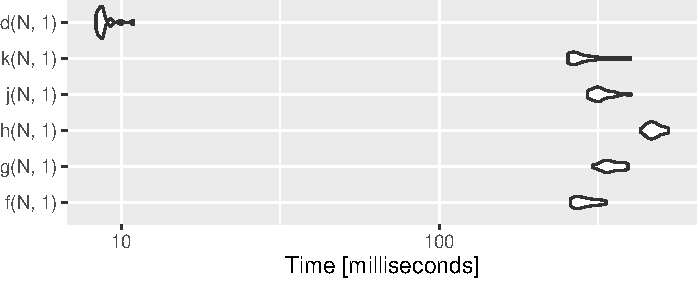
\includegraphics{lec5_functions_recursion_memoization_benchmarking_files/figure-beamer/compare_ggplot2-1.pdf}

\end{frame}

\begin{frame}{Summary of Benchmarking}

\begin{itemize}
\tightlist
\item
  Covered usage reasons for benchmarking code
\item
  Discussed areas of concern for obtaining benchmarks.
\end{itemize}

\end{frame}

\begin{frame}{Memoization}

Coming up next\ldots{} \textbf{Memoization} in R!

\end{frame}

\begin{frame}{Caching Values is Memoization}

One of the common themes of this course is caching or storing values to
be reused later during a computation.

\begin{itemize}
\item
  This is exactly the definition of \textbf{memoization}.
\item
  Memoization is key to a lot of intense statistical computations. A
  recent entry on this can be found as a response to a question on
  \href{http://stackoverflow.com/a/36973875/1345455}{StackOverflow}.
\end{itemize}

\end{frame}

\begin{frame}{Memoization in Depth}

The goal of memoization is to cache function results under given
parameters and reuse them at a later time.

\begin{itemize}
\tightlist
\item
  To cache the value of the computation, a key is created that relates
  the function and the parameters used within it.
\item
  Thus, after one calculation under the given parameters the function no
  longer needs to recalculate the same result again if called for any
  other sequence in the computation.
\item
  The reason why is the result can just retrieve the value from the
  cache.
\end{itemize}

\textbf{Note} This is particularly relevant for the recursive structure
set up.

\end{frame}

\begin{frame}[fragile]{Memoization in R}

Hadley Wickham, Jim Hester, and Kirill Müller have created phenomenal
package called
\href{https://cran.r-project.org/web/packages/memoise/index.html}{\texttt{memoise}}.

\begin{itemize}
\tightlist
\item
  The package brings in the ability to memoization functions with very
  little work.
\end{itemize}

\end{frame}

\begin{frame}{Fibonacci Sequence}

The Fibonacci Sequence is a famous series that traditionally looks like
so:

\[1, 1, 2, 3, 5, 8, 13, 21 \]

The mathematical formulation is known as:

\[ F\left( n \right) = F\left( {n - 1} \right) + F\left( {n - 2} \right)\]

where \(F(1) = 1\) and \(F(2) = 1\).

\end{frame}

\begin{frame}[fragile]{Example Fibonacci Sequence}

We can write the Fibonacci Sequence like so:

\begin{Shaded}
\begin{Highlighting}[]
\NormalTok{fibonacci =}\StringTok{ }\NormalTok{function(n) \{}
   \NormalTok{if (n <}\StringTok{ }\DecValTok{2}\NormalTok{) \{}
     \KeywordTok{return}\NormalTok{(}\DecValTok{1}\NormalTok{)}
   \NormalTok{\}}
  
   \KeywordTok{return}\NormalTok{(}\KeywordTok{fibonacci}\NormalTok{(n}\DecValTok{-2}\NormalTok{) +}\StringTok{ }\KeywordTok{fibonacci}\NormalTok{(n}\DecValTok{-1}\NormalTok{))}
\NormalTok{\}}
\end{Highlighting}
\end{Shaded}

\end{frame}

\begin{frame}[fragile]{Example Memoization}

To memoize the Fibonacci function, we need to wrap place the function
name in \texttt{memoise()}

\begin{Shaded}
\begin{Highlighting}[]
\KeywordTok{library}\NormalTok{(}\StringTok{"memoise"}\NormalTok{)}
\NormalTok{mem_fib =}\StringTok{ }\KeywordTok{memoise}\NormalTok{(fibonacci)}
\end{Highlighting}
\end{Shaded}

We then refer to the memoized function just like normal previously, e.g.

\begin{Shaded}
\begin{Highlighting}[]
\KeywordTok{fibonacci}\NormalTok{(}\DecValTok{5}\NormalTok{) }\CommentTok{# Normal}
\end{Highlighting}
\end{Shaded}

\begin{verbatim}
## [1] 8
\end{verbatim}

\begin{Shaded}
\begin{Highlighting}[]
\KeywordTok{mem_fib}\NormalTok{(}\DecValTok{5}\NormalTok{)   }\CommentTok{# Memoized}
\end{Highlighting}
\end{Shaded}

\begin{verbatim}
## [1] 8
\end{verbatim}

\end{frame}

\begin{frame}[fragile]{Benchmarks}

When we write it this way, we gain speed due to the cache given by
memoization being used. e.g.

\begin{Shaded}
\begin{Highlighting}[]
\KeywordTok{system.time}\NormalTok{(\{}\KeywordTok{fibonacci}\NormalTok{(}\DecValTok{35}\NormalTok{)\}) }\CommentTok{# Normal}
\end{Highlighting}
\end{Shaded}

\begin{verbatim}
##    user  system elapsed 
##  20.728   0.066  21.060
\end{verbatim}

\begin{Shaded}
\begin{Highlighting}[]
\KeywordTok{system.time}\NormalTok{(\{}\KeywordTok{mem_fib}\NormalTok{(}\DecValTok{35}\NormalTok{)\})   }\CommentTok{# Memoized}
\end{Highlighting}
\end{Shaded}

\begin{verbatim}
##    user  system elapsed 
##  20.748   0.049  21.087
\end{verbatim}

\end{frame}

\begin{frame}[fragile]{Benchmarks}

\begin{Shaded}
\begin{Highlighting}[]
\KeywordTok{system.time}\NormalTok{(\{}\KeywordTok{fibonacci}\NormalTok{(}\DecValTok{25}\NormalTok{)\}) }\CommentTok{# Normal}
\end{Highlighting}
\end{Shaded}

\begin{verbatim}
##    user  system elapsed 
##   0.166   0.000   0.168
\end{verbatim}

\begin{Shaded}
\begin{Highlighting}[]
\KeywordTok{system.time}\NormalTok{(\{}\KeywordTok{mem_fib}\NormalTok{(}\DecValTok{25}\NormalTok{)\})   }\CommentTok{# Memoized}
\end{Highlighting}
\end{Shaded}

\begin{verbatim}
##    user  system elapsed 
##   0.168   0.000   0.171
\end{verbatim}

\end{frame}

\begin{frame}[fragile]{Clear the Cache}

To remove memoization, use \texttt{forget()}

\begin{Shaded}
\begin{Highlighting}[]
\KeywordTok{forget}\NormalTok{(}\KeywordTok{mem_fib}\NormalTok{(}\DecValTok{35}\NormalTok{))}
\end{Highlighting}
\end{Shaded}

\begin{verbatim}
## [1] FALSE
\end{verbatim}

\textbf{Note}

You will have to declare it again.

\end{frame}

\begin{frame}{Summary of memoization}

\begin{itemize}
\tightlist
\item
  Memoization is used for speed
\item
  Very helpful for recursive functions
\item
  Watch the catch
\end{itemize}

\end{frame}
